\paragraph{Training-set size (H5): supported.} Table~\ref{tab:sweep} and Fig.~\ref{fig:sweep} vary $N$ from 250 to 4000 on L15\_A4\_K2 and L20\_A20\_K1 ($N=1000$ comes from the main group). The registered test concerns the $K=2$ task: the Pairwise$-$Additive Spearman gap there is larger at $N=4000$ ($0.311$) than at $N=250$ ($0.067$), and grows at every step in between; on L20\_A20\_K1 it grows from $0.005$ to $0.091$. Regarding H3, the networks stay below pairwise ridge at every $N$ on both tasks. On L15\_A4\_K2 they are indistinguishable from additive ridge at $N=500$ ($0.284$, $0.283$ versus $0.285$) and close the distance to pairwise ridge at $N=4000$ ($0.616$ and $0.628$ versus $0.669$, gaps of $0.053$ and $0.042$). On L20\_A20\_K1, however, they are at or below additive ridge at every $N$ (the one exception, MLP $0.070$ versus $0.068$ at $N=500$, is far inside the seed spread of Fig.~\ref{fig:sweep}), the best score at $N=4000$ is only $0.302$, and their distance to pairwise ridge does not shrink ($0.162$ and $0.192$ versus $0.302$). So H3 held at every $N$ we ran; the sweep suggests the gap may close with more data on L15\_A4\_K2, but $N>4000$ was not run and only two tasks were swept.

\begin{table}[t]\centering\caption{Test Spearman versus training size $N$ (mean of 5 seeds).}\label{tab:sweep}\resizebox{\columnwidth}{!}{\begin{tabular}{lrrrrr}
\toprule
Task & $N$ & Add. & Pair. & CNN & MLP\\
\midrule
L15\_A4\_K2 & 250 & 0.234 & 0.301 & 0.232 & 0.234\\
L15\_A4\_K2 & 500 & 0.285 & 0.374 & 0.284 & 0.283\\
L15\_A4\_K2 & 1000 & 0.310 & 0.508 & 0.384 & 0.383\\
L15\_A4\_K2 & 2000 & 0.335 & 0.594 & 0.515 & 0.517\\
L15\_A4\_K2 & 4000 & 0.358 & 0.669 & 0.616 & 0.628\\
\midrule
L20\_A20\_K1 & 250 & 0.065 & 0.070 & 0.048 & 0.058\\
L20\_A20\_K1 & 500 & 0.068 & 0.091 & 0.060 & 0.070\\
L20\_A20\_K1 & 1000 & 0.110 & 0.138 & 0.077 & 0.090\\
L20\_A20\_K1 & 2000 & 0.163 & 0.215 & 0.115 & 0.140\\
L20\_A20\_K1 & 4000 & 0.211 & 0.302 & 0.162 & 0.192\\
\bottomrule
\end{tabular}
}\end{table}
\begin{figure}[t]\centering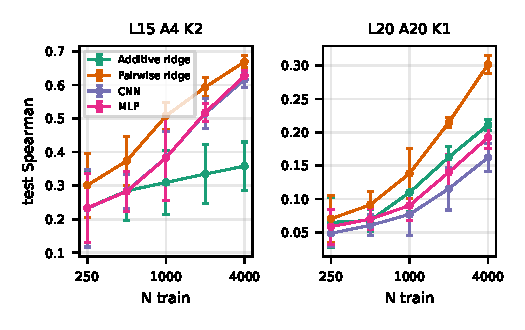
\includegraphics[width=\columnwidth]{generated/fig_sweep_n.pdf}\caption{Test Spearman versus $N$ (mean $\pm$ SD, 5 seeds).}\label{fig:sweep}\end{figure}

\paragraph{Pair-feature ablations.} Table~\ref{tab:abl} compares tuned Pairwise ridge with (i) the penalty ratio fixed at $r=1$ and (ii) pair features restricted to the true interaction graph (an oracle). Fixing $r=1$ matters only where pair features carry no signal: at L20\_A20\_K0 it costs $0.995\to0.897$; elsewhere the differences ($\le0.012$) are within one seed standard deviation. The oracle graph helps in two cells: $0.508\to0.621$ on L15\_A4\_K2 and $0.138\to0.250$ on L20\_A20\_K1; it is at ceiling ($1.000$) at $K\le1$ for (15,4). Even then L15\_A4\_K2 stays at $0.621$, below the level that $K=1$ reaches, which is consistent with (but not proof of) order-3 terms that no pairwise model can capture; and at $K=4$ nothing helps ($0.084$ at best). We did not run a three-way-interaction model, so the order-3 explanation is untested. Knowing which pairs interact was thus worth about $0.11$ Spearman in those two cells and at most $0.005$ in the other six; this is an upper reference for what pair selection could add in this simulator, obtained with information a practitioner lacks.

\begin{table}[t]\centering\caption{Pairwise-ridge ablations, test Spearman, mean $\pm$ SD over 5 seeds ($N=1000$).}\label{tab:abl}\resizebox{\columnwidth}{!}{\begin{tabular}{lrrr}
\toprule
Task & Pair. (tuned $r$) & Pair. ($r{=}1$) & Pair. (oracle graph)\\
\midrule
L15\_A4\_K0 & 1.000 $\pm$ 0.000 & 1.000 $\pm$ 0.000 & 1.000 $\pm$ 0.000\\
L15\_A4\_K1 & 0.998 $\pm$ 0.002 & 0.998 $\pm$ 0.002 & 1.000 $\pm$ 0.000\\
L15\_A4\_K2 & 0.508 $\pm$ 0.040 & 0.500 $\pm$ 0.048 & 0.621 $\pm$ 0.024\\
L15\_A4\_K4 & 0.080 $\pm$ 0.019 & 0.079 $\pm$ 0.031 & 0.084 $\pm$ 0.028\\
L20\_A20\_K0 & 0.995 $\pm$ 0.000 & 0.897 $\pm$ 0.007 & 1.000 $\pm$ 0.000\\
L20\_A20\_K1 & 0.138 $\pm$ 0.038 & 0.150 $\pm$ 0.025 & 0.250 $\pm$ 0.024\\
L20\_A20\_K2 & 0.025 $\pm$ 0.015 & 0.028 $\pm$ 0.017 & 0.029 $\pm$ 0.013\\
L20\_A20\_K4 & 0.014 $\pm$ 0.008 & 0.013 $\pm$ 0.007 & 0.015 $\pm$ 0.008\\
\bottomrule
\end{tabular}
}\end{table}
